\begin{figure*}[h]
  \centering
  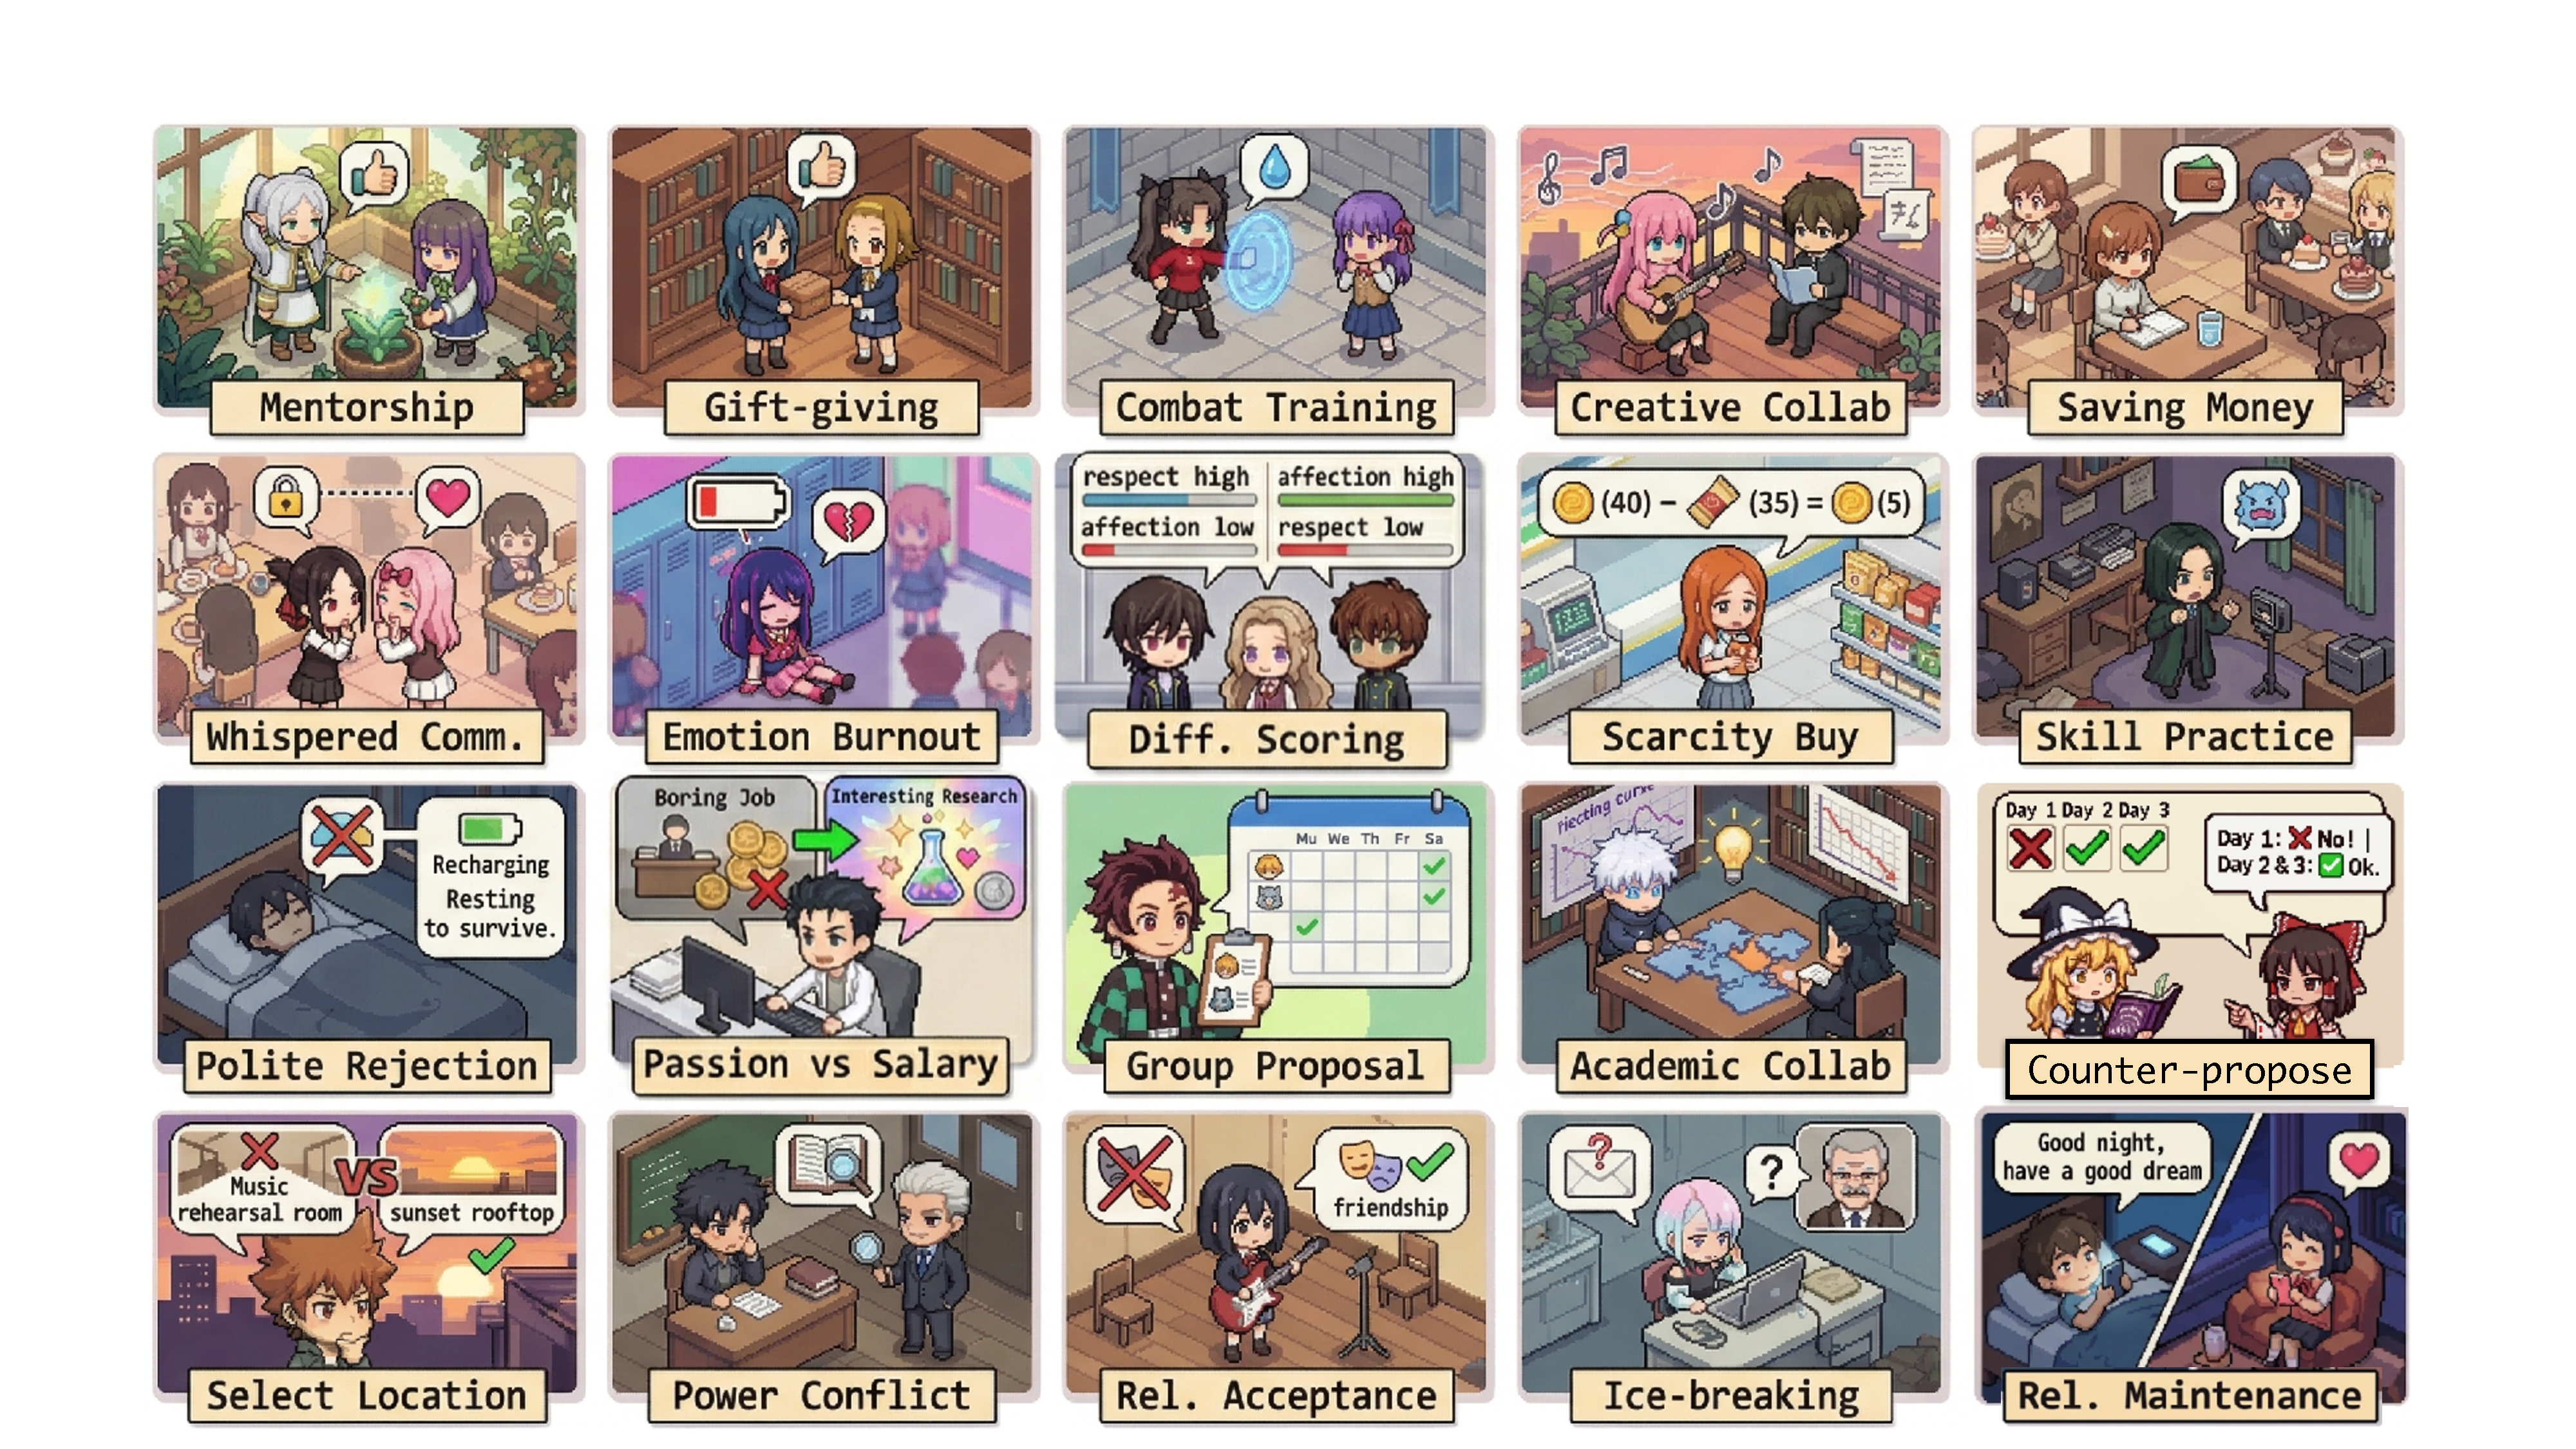
\includegraphics[width=0.9\textwidth]{Figures/agentopia-exe.pdf}
  \caption{Illustration of emergent behaviors observed in \method simulations.
  Each scene depicts a real behavioral pattern documented in our case studies (Tables~\ref{tab:planning}--\ref{tab:emergent}).
  Without explicit scripting, agents autonomously develop diverse behavioral patterns reflecting agents' intelligence in social life.
  }
  \label{fig:emergent-behaviors}
\end{figure*}

\vspace*{-10pt}

\section{Introduction}
\label{sec:intro}



Humans learn from social environments~\citep{vygotsky1978mind}, and large language models (LLMs) learn from humans.
As LLMs advance, how to better understand and simulate human thought, emotion, and behavioral patterns has become an important research problem, which is known as LLM-based persona simulation, or role-playing~\citep{chen2024from}.
LLM role-playing is widely adopted in AI companions, digital games, and content creation~\citep{shao2023character, zhou2023characterglm}, such as \textit{Whispers from the Star}.~\footnote{\url{https://wfts.anuttacon.com/}}
However, faithfully aligning LLMs with human mind remains a challenge.
As human data approaches exhaustion,
future AI agents need to learn primarily through experience~\citep{silver2025era}.
This motivates a straightforward idea:
since humans learn and grow through social lives in human societies~\citep{maslow1943theory},
\textit{can agents do the same --- learning, growing, and becoming more human-like through lives in agent societies?}
This requires building an agent society
that supports long-term life simulation,
encourages social behaviors such as growth, competition, intimate relationships, and resource allocation,
and provides rewards that mirror human well-being for optimization.


Prior work has studied LLM-based social simulation and persona simulation in short-term settings.
For social simulation,
previous efforts have built prototypes of agent societies,
\eg, Generative Agents~\citep{park2023generative} and Aivilization~\citep{fan2026aivilization}.
However, these works primarily focus on low-level operations
such as \dq{collecting 2 wheat to craft 1 flour},
instead of long-term social dynamics, keeping simulations at the scale of days.
For persona simulation,
existing efforts focuses on role-playing within individual conversations~\citep{chen2024from, shao2023character},
emphasizing anthropomorphism, character fidelity, and user engagement, 
rather than life simulation of agents themselves.
These methods rely heavily on human data for optimization~\citep{wang2025coser, liu-etal-2025-cogdual, du2026her}, which is costly to collect and difficult to scale up, and thus remain insufficient to deeply align LLMs with human cognition.
Overall, existing research only study simulation at the scale of days or single conversations,
leaving long-term life simulation unexplored.


In this paper, we present \method,
a framework for long-term life simulation in multi-agent societies,
where agents autonomously simulate years of human social lives, as illustrated in Figure~\ref{fig:framework}.

In \method, agents build social relationships,
develop personal skills,
set and accomplish goals,
develop and fulfill needs,
and engage in economic activities.
\method focuses on social interactions rather than low-level operations.
The framework is characterized by several key features:
\textit{(1)} \method defines \textit{life reward} to model human well-being,
representing social standing, subjective fulfillment, and economic status.
\textit{(2)} \method employs an \textit{environment model} to serve as a generative environment engine that orchestrates the simulation,
avoiding the need to hard-code massive rules.
It serves multiple purposes including
verifying agent responses against role-playing principles,
providing feedback on agent behaviors, and creating and scheduling events.
\textit{(3)} \method implements a comprehensive \textit{context management} mechanism to provide agents with sufficient context, and equips agents with \textit{memory files}, a file-system-based long-term memory that agents autonomously manage what to remember, update, or discard.
Furthermore, leveraging simulation and reward in \method, we propose \textit{life reward training} optimize LLMs via rejection sampling,
improving LLMs in anthropomorphism, role-playing ability, and intelligence in social life.

Towards long-term life simulation,
\method introduces a carefully designed simulation procedure.
It aims to model as many real-world social interactions as possible within a unified framework.
The core challenge is that LLMs generate by turns, 
while humans can perceive and act at any time.
Hence, we structure time into discrete units, allowing concurrent yet ordered interactions.
\method uses the \textit{week} as its basic time unit.
Each week consists of four stages:
\textit{(1)} \textit{Plan},
\textit{(2)} \textit{Contact} others and arrange schedules,
\textit{(3)} carry out solo or group \textit{Activity} over subsequent days,
and \textit{(4)} \textit{Review} the week's experiences.
The \textit{year} serves as a larger cycle.
At the end of each year, 
\method updates agents' profiles , 
allows agents to apply for new careers, 
and calculates life rewards for them.


To validate this framework,
we create three diverse fictional worlds and conduct simulations.
Each world contains 100 agents running for 10 simulated years.
This scale is orders of magnitude larger than prior studies.
We conduct multi-faceted analyses of these simulations,
such as reward and behavior analysis,
social relationship evolution,
and social mobility.
We also conduct extensive case studies to observe emergent behaviors in agent societies, as shown in Figure~\ref{fig:emergent-behaviors}.
Besides, we use \method as an arena to compare different models' performance.
Subsequently, we demonstrate the effectiveness of life reward training.
The trained model demonstrates improved overall well-being in simulation,
including improved social relationships, higher subjective fulfillment, and better economic gains.
Furthermore, the improvements generalize to enhanced anthropomorphism and role-playing ability,
achieving +15.6\% performance gain on CoSER Test~\citep{wang2025coser}, a downstream role-playing benchmark.


Our contributions are summarized as follows:
\begin{enumerate}
  \item We introduce \method, a system for long-term life simulation in agent societies.
        Compared to prior work,
        \method extends the scale of life simulation from days to years for the first time,
        enabling long-term social dynamics 
        such as personal growth, relationship building, life planning, and, \etc
  \item Based on \method, we define \textit{life reward} to mirror human well-being, and propose \textit{life reward training} that fine-tunes LLMs on high-advantage agent experiences, without relying on human data.
       
  \item We conduct extensive experiments on \method,
        including comprehensive analyses and case studies on agents' social behaviors.
        We also validate the effectiveness of life reward training,
        which improves in-simulation well-being
        as well as anthropomorphism and role-playing ability in downstream evaluation.
\end{enumerate}

\begin{figure*}[t]
    \centering
    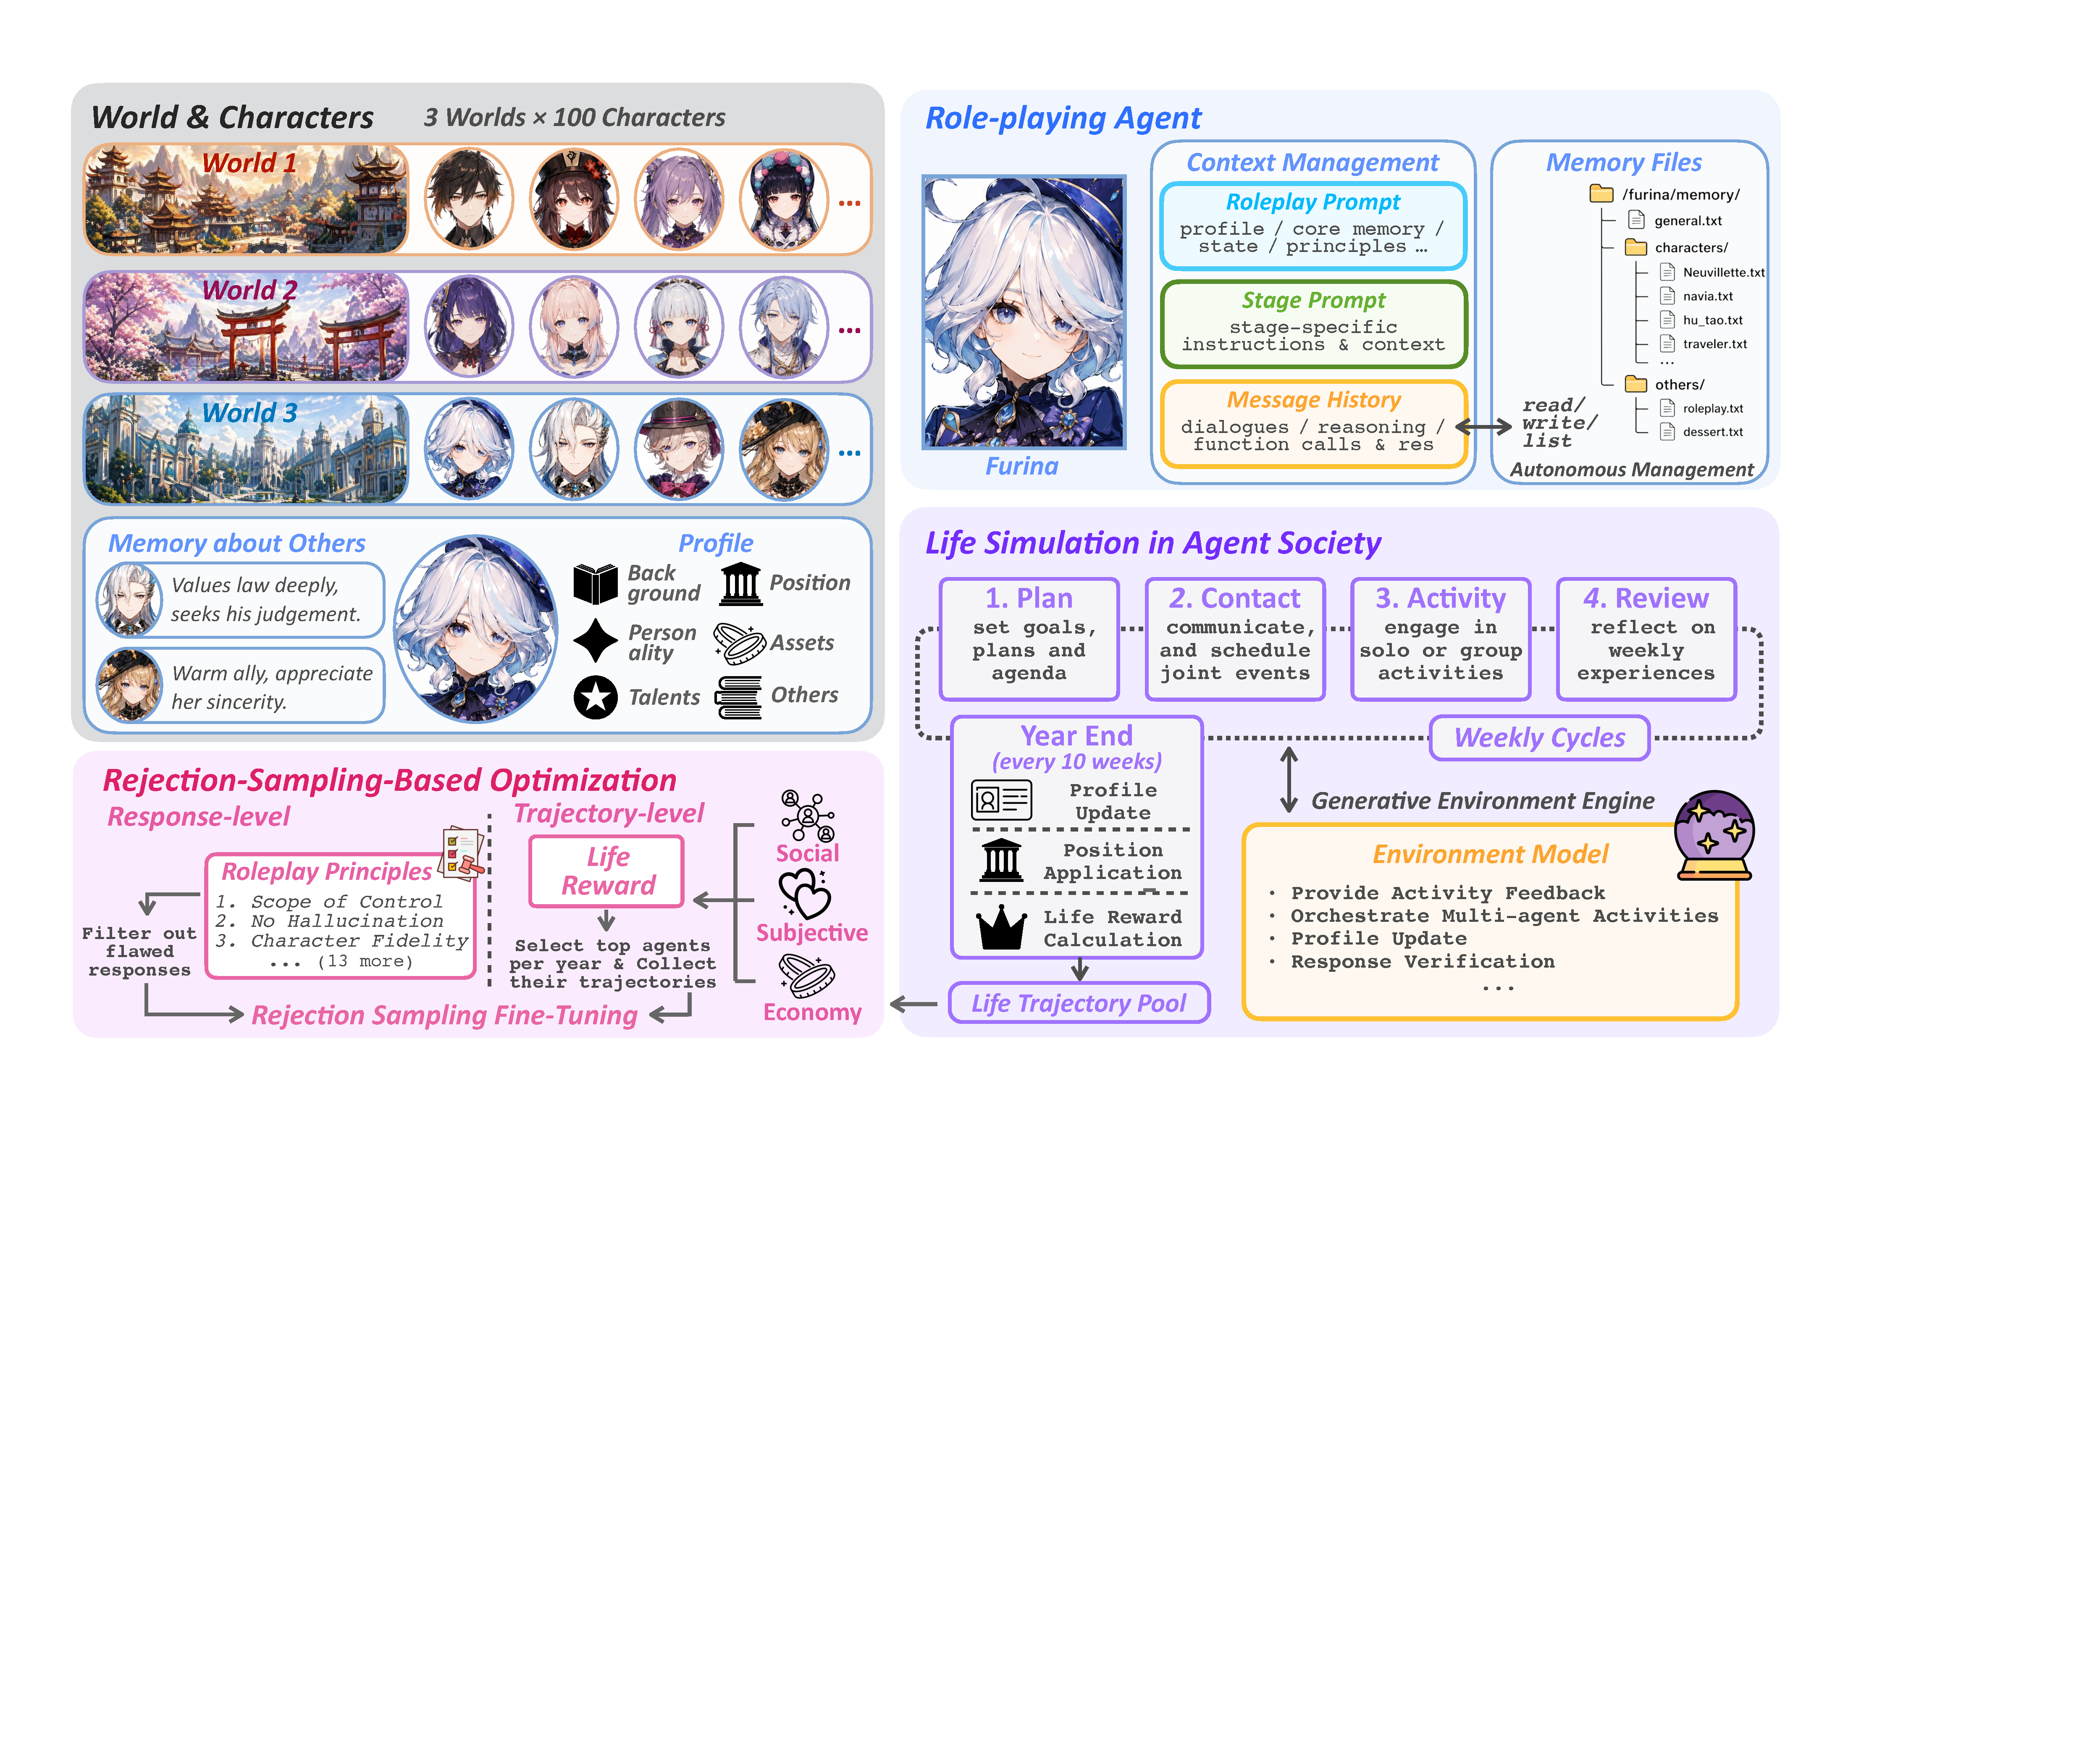
\includegraphics[width=\textwidth]{Figures/Agentopia-main.pdf}
    \caption{Overview of \method: world and character construction (\S~\ref{app:creation}), role-playing agent (\S~\ref{sec:agent_design}), life simulation in agent society (\S~\ref{sec:simulation_procedure}), and life reward training (\S~\ref{sec:training_data}).}
    \label{fig:framework}
\end{figure*}
